
\hypertarget{menu_encoding}{}
\section{Encoding}
\index{encoding}

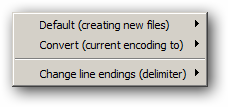
\includegraphics[scale=0.50]{./res/menu_encoding.png}\\

\begin{scriptsize}\begin{tabularx}{\textwidth}{>{\hsize=0.4\hsize}X>{\hsize=0.6\hsize}X}\\
    \hline
    \textbf{Option} & \textbf{Description} \\
    \hline
    Default (creating new files) & \textit{\htmladdnormallink{See options ...}{\#menu\_encoding\_default}} \\
    Convert (current encoding to) & \textit{\htmladdnormallink{See options ...}{\#menu\_encoding\_convert}} \\
    Change line ending (delimiter) & \textit{\htmladdnormallink{See options ...}{\#menu\_encoding\_delimiter}} \\
    \hline
  \end{tabularx}\end{scriptsize}

\hypertarget{menu_encoding_default}{}
\subsubsection{Default (creating new files):}\\
\index{encoding!ANSI}
\index{encoding!UTF-8}
\index{encoding!UTF16-LE}
\index{encoding!UTF16-BE}

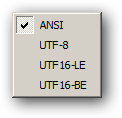
\includegraphics[scale=0.50]{./res/menu_encoding_default.png}\\

\begin{scriptsize}\begin{tabularx}{\textwidth}{>{\hsize=0.3\hsize}X>{\hsize=0.7\hsize}X}\\
    \hline
    \textbf{Option} & \textbf{Description} \\
    \hline
    ANSI & Sets encoding to ANSI \\
    UTF-8 & Sets encoding to UTF-8 \\
    UTF16-LE & Sets encoding to UTF16-LE \\
    UTF16-BE & Sets encoding to UTF16-BE \\
    \hline
  \end{tabularx}\end{scriptsize}

\hypertarget{menu_encoding_convert}{}
\subsubsection{Convert (current encoding to):}\\
\index{encoding!ANSI}
\index{encoding!UTF-8}
\index{encoding!UTF16-LE}
\index{encoding!UTF16-BE}

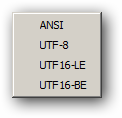
\includegraphics[scale=0.50]{./res/menu_encoding_convert.png}\\

\begin{scriptsize}\begin{tabularx}{\textwidth}{>{\hsize=0.3\hsize}X>{\hsize=0.7\hsize}X}\\
    \hline
    \textbf{Option} & \textbf{Description} \\
    \hline
    ANSI & Converts current encoding to ANSI \\
    UTF-8 & Converts current encoding to UTF-8 \\
    UTF16-LE & Converts current encoding to UTF16-LE \\
    UTF16-BE & Converts current encoding to UTF16-BE \\
    \hline
  \end{tabularx}\end{scriptsize}

\hypertarget{menu_encoding_delimiter}{}
\subsubsection{Change line ending (delimiter):}\\
\index{delimiter}
\index{delimiter!WIN (CR+LF)}
\index{delimiter!MAC (CR)}
\index{delimiter!UNIX (LF)}

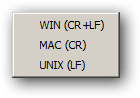
\includegraphics[scale=0.50]{./res/menu_encoding_delimiter.png}\\

\begin{scriptsize}\begin{tabularx}{\textwidth}{>{\hsize=0.3\hsize}X>{\hsize=0.7\hsize}X}\\
    \hline
    \textbf{Option} & \textbf{Description} \\
    \hline
    WIN (CR+LF) & Changes line endings (delimiter) to WIN (CR+LF) \\
    MAC (CR) & Changes line endings (delimiter) to MAC (CR) \\
    UNIX (LF) & Changes line endings (delimiter) to UNIX (LF) \\
    \hline
  \end{tabularx}\end{scriptsize}
